% 2017 全国Ⅰ卷 理18/文18：四棱锥 P-ABCD（AB∥CD，∠BAP=∠CDP=90°）
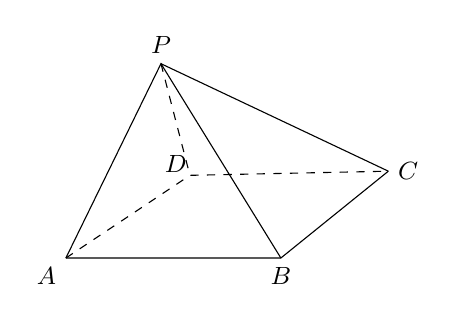
\begin{tikzpicture}[scale=1.05, font=\small]
  \coordinate (P) at (1.15,2.35);
  \coordinate (A) at (0,0);
  \coordinate (B) at (2.6,0);
  \coordinate (C) at (3.9,1.05);
  \coordinate (D) at (1.5,1.0);
  \draw (A) -- (B) -- (C);
  \draw (A) -- (P) -- (B);
  \draw (P) -- (C);
  \draw[dashed] (A) -- (D) -- (C);
  \draw[dashed] (P) -- (D);
  \node[above] at (P) {$P$};
  \node[below left] at (A) {$A$};
  \node[below] at (B) {$B$};
  \node[right] at (C) {$C$};
  \node[above left, inner sep=1pt] at (D) {$D$};
\end{tikzpicture}
